\documentclass[10pt]{article}
\usepackage[letterpaper,top=0.55in,bottom=0.58in,left=0.62in,right=0.62in]{geometry}
\usepackage[T1]{fontenc}
\usepackage[utf8]{inputenc}
\usepackage{lmodern}
\usepackage{microtype}
\usepackage{graphicx}
\usepackage{booktabs}
\usepackage{array}
\usepackage{enumitem}
\usepackage{titlesec}
\usepackage{xcolor}
\usepackage{tikz}
\usetikzlibrary{arrows.meta,positioning,shapes.geometric,fit}
\usepackage{amsmath,amssymb}
\usepackage{hyperref}
\usepackage{multicol}
\usepackage{caption}

\definecolor{ink}{HTML}{17243A}
\definecolor{blue}{HTML}{1B5EA7}
\definecolor{cyan}{HTML}{DCEFF6}
\definecolor{gold}{HTML}{C58B1B}
\definecolor{soft}{HTML}{F3F5F7}
\hypersetup{colorlinks=true,linkcolor=blue,urlcolor=blue,citecolor=blue}
\color{ink}
\setlength{\parindent}{0pt}
\setlength{\parskip}{2.2pt}
\setlength{\columnsep}{14pt}
\setlist[itemize]{leftmargin=1.3em,itemsep=0pt,topsep=2pt,parsep=0pt}
\setlist[enumerate]{leftmargin=1.5em,itemsep=0pt,topsep=2pt,parsep=0pt}
\titleformat{\section}{\large\bfseries\color{blue}}{}{0pt}{}[\vspace{-2pt}\color{cyan}\titlerule]
\titleformat{\subsection}{\normalsize\bfseries\color{ink}}{}{0pt}{}
\titlespacing*{\section}{0pt}{5pt}{3pt}
\titlespacing*{\subsection}{0pt}{4pt}{1pt}
\captionsetup{font=footnotesize,labelfont=bf,skip=2pt}
\pagestyle{plain}

\newcommand{\armT}{\textsc{Time}}
\newcommand{\armC}{\textsc{Cost}}
\newcommand{\armB}{\textsc{Baseline}}
\newcommand{\E}{\mathbb{E}}

\begin{document}

\begin{center}
{\LARGE\bfseries Faces or Facts?}\par
\vspace{1pt}
{\large Experimental Evidence on Time Pressure, Information Costs, and Gender Bias in Electoral Choice}\par
\vspace{3pt}
{\normalsize Nayssa Alejandra Mar\'in D\'iaz \quad Andrea Canales \quad H\'ector Bahamonde}\par
\vspace{1pt}
{\small Design and analysis proposal --- work in progress --- 30 September 2026}
\end{center}

\vspace{-3pt}
\noindent\colorbox{cyan}{\parbox{0.978\linewidth}{\small
\textbf{Abstract.} How do visual impressions compete with substantive political information when voters choose between candidates? We field a three-arm online visual conjoint experiment using photographs and programmatic information from Colombian electoral data. Eligible adults outside Colombia complete five practice and fifteen consequential paired-profile choices. The experiment independently assigns respondents to a 10-second deadline, a cognitive cost for revealing political information, or an unconstrained baseline. Candidate pairs and left-right positions are randomized within respondents. We record vote choice, information-reveal behavior, response time, treatment exposure, and the complete candidate-source row shown in every task. The design identifies intention-to-treat effects of decision environments and causal effects of assigning complete candidate profiles. Because the attributes within a real candidate profile are not independently randomized, gender-, ideology-, and appearance-based contrasts are interpreted as effects of bundled profiles or as descriptive heterogeneity, not conventional attribute-level AMCEs. The project contributes a process-trace account of when voters rely on faces rather than facts and whether these environments reproduce gendered electoral inequalities.}}

\section{Problem, literature, and contribution}

Candidate photographs can shape political choice after extremely brief exposure. Perceived competence from faces predicts election outcomes (Todorov et al. 2005), photographs operate as cues in low-information contests (Banducci et al. 2008), and appearance predicts electoral success across established and newer democracies (Rosar et al. 2008; Berggren et al. 2010; Lawson et al. 2010). Media exposure can intensify this channel among less informed voters (Lenz and Lawson 2011). Appearance does more than communicate attractiveness: faces invite inferences about competence, trustworthiness, ideology, party, status, and threat (Mattes et al. 2010; Herrmann and Shikano 2016; Olivola et al. 2018). Recent evidence shows that voters reward candidates who look upper class and impose a particularly large penalty on women who look working class (Bahamonde and Sarpila 2024). Together, this literature presents appearance as a politically consequential heuristic rather than superficial noise.

Yet ``looks matter'' is not a complete causal account. Voters can inspect policy information, and the decision environment determines whether doing so is feasible or attractive. General work on electoral heuristics emphasizes that shortcuts can reduce effort but sometimes distort judgment (Lau and Redlawsk 2001). Candidate gender changes both the amount and type of information voters seek (Ditonto, Hamilton, and Redlawsk 2014), while identical facial impressions can have different electoral implications for men and women (Ditonto and Mattes 2018). Time pressure encourages less deliberative strategies, and experimental evidence shows that it can alter voting behavior itself (Al\'os-Ferrer and Garagnani 2022). The literature therefore implies a mechanism---visual cues become relatively influential when attention is scarce or facts are costly---but has rarely observed the full chain from randomized decision environment, through information acquisition, to candidate choice.

This study joins these literatures in one behavioral design. It contributes (1) a direct comparison of temporal scarcity and an explicit information-acquisition cost; (2) click-level measurement of whether substantive information was requested; (3) repeated choices between authentic candidate profiles assembled from Colombian electoral data; and (4) a gender-and-inequality perspective that moves beyond attractiveness alone. It also separates what the experiment truly randomizes from what it merely measures. Standard conjoint AMCEs require independently randomized attribute levels (Hainmueller, Hopkins, and Yamamoto 2014). Here, the photograph, gender, ideology, electoral history, and facial measurements travel together as a real candidate profile. Our primary causal claims therefore concern the assigned decision environment and the randomly displayed \emph{whole profiles}; analyses of component features are explicitly secondary.

\section{Design and implementation}

\textbf{Population and screening.} The planned sample is 462 adults aged 18--65, balanced across men and women and allocated approximately equally across the three arms ($154$ per arm). To minimize recognition and prior Colombian political knowledge, respondents must neither be Colombian nationals nor currently reside in Colombia, and must report never having lived in Colombia. Residence, nationality, and prior residence are asked sequentially so that an ineligible person exits immediately. Age, gender identity, occupation, education, turnout, political interest, discussion frequency, and left-right self-placement are then collected on one page.

\textbf{Stimuli and repeated choice.} The deployed candidate pool contains 71 profiles with nonmissing programmatic text in \texttt{base\_final\_merged.csv}. Each respondent receives 40 distinct profile assignments---two per round---randomized without replacement into five practice and fifteen analysis rounds. Within each round, the pair and left-right placement are randomized. A profile shows the candidate photograph and a button that can reveal the Spanish \texttt{Texto} field (ideology plus policy priorities). The binary outcome is the selected candidate. Fifteen main tasks are defensible in light of experimental evidence that substantially larger conjoint batteries produce only limited average satisficing in comparable online settings (Bansak et al. 2018); practice rounds are excluded from confirmatory estimates.

\begin{figure}[h!]
\centering
\begin{minipage}[t]{0.475\linewidth}
\centering
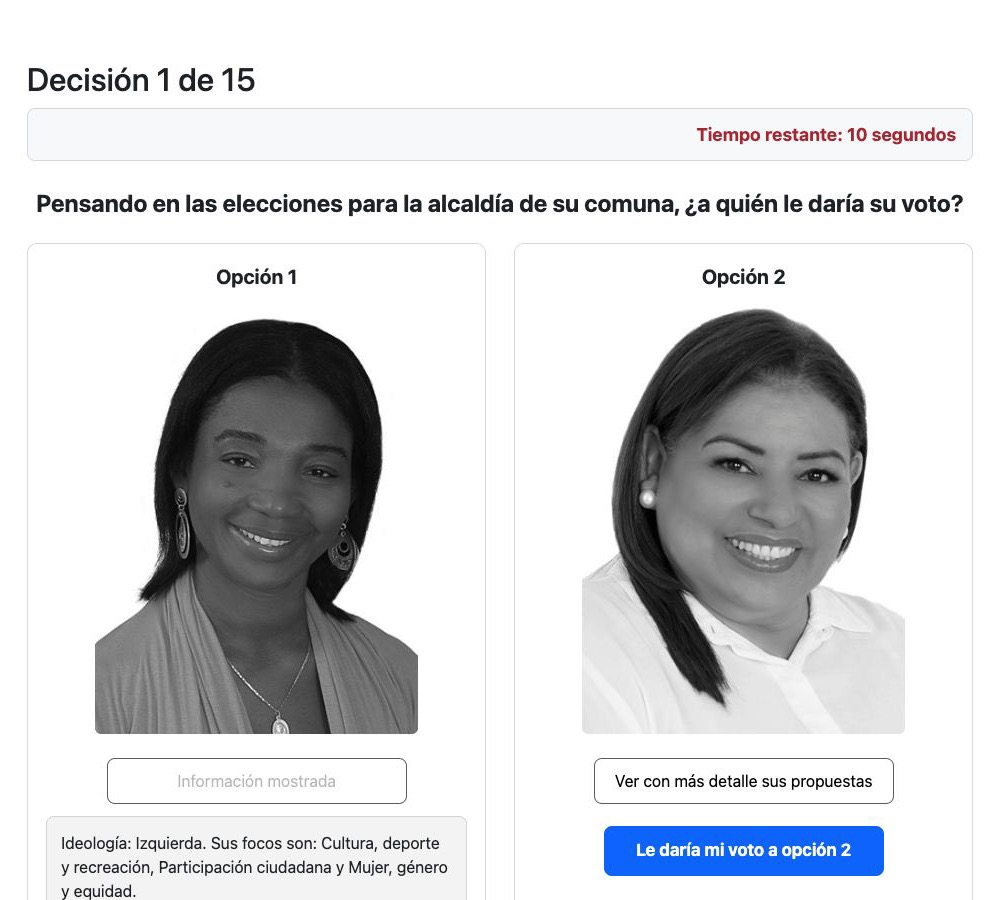
\includegraphics[width=\linewidth,height=2.12in,keepaspectratio]{assets/task_example.jpg}
\caption*{\textbf{A. Task interface.} A live oTree task using Colombian candidate photographs; the left profile's programmatic text has been revealed.}
\end{minipage}\hfill
\begin{minipage}[t]{0.50\linewidth}
\centering
\resizebox{\linewidth}{!}{%
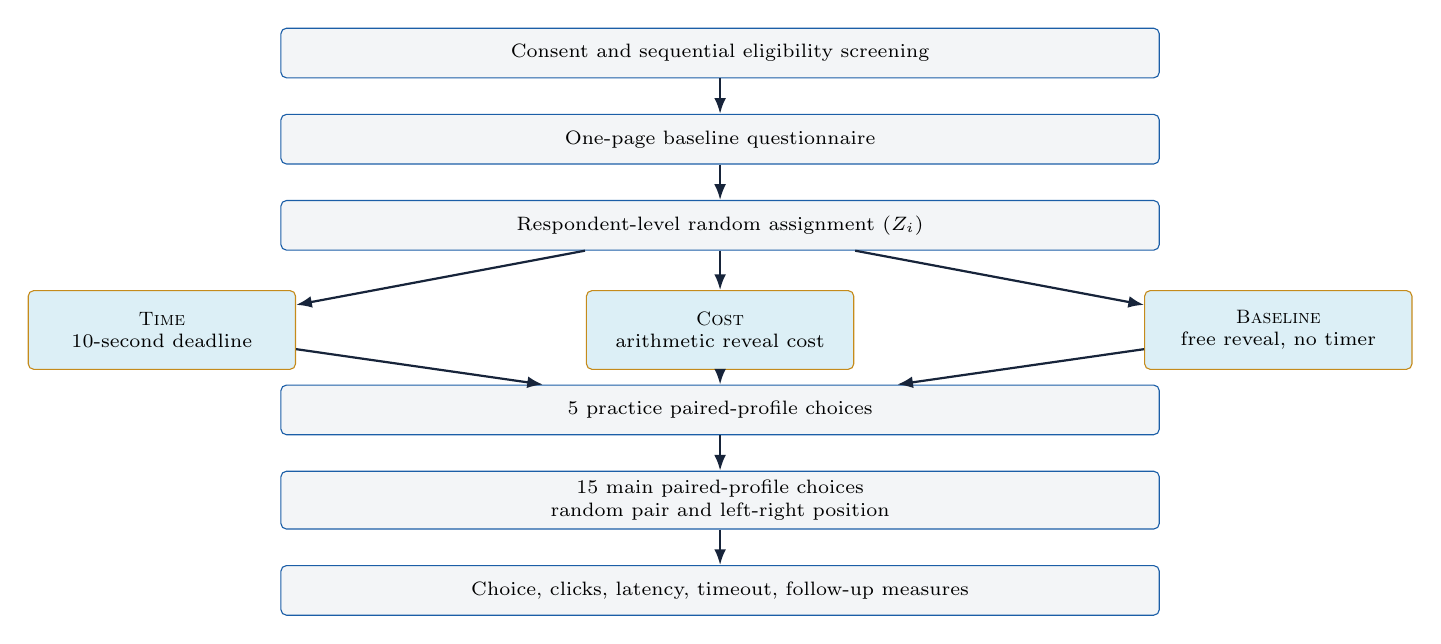
\begin{tikzpicture}[
  node distance=4.5mm and 5mm,
  box/.style={rounded corners=2pt,draw=blue,fill=soft,minimum width=0.92\linewidth,minimum height=6.3mm,align=center,font=\scriptsize},
  arm/.style={rounded corners=2pt,draw=gold,fill=cyan,minimum width=0.28\linewidth,minimum height=10mm,align=center,font=\scriptsize},
  arr/.style={-{Latex[length=2mm]},thick,draw=ink}
]
\node[box] (screen) {Consent and sequential eligibility screening};
\node[box,below=of screen] (survey) {One-page baseline questionnaire};
\node[box,below=of survey] (rand) {Respondent-level random assignment ($Z_i$)};
\node[arm,below left=5mm and -2mm of rand] (time) {\armT\\10-second deadline};
\node[arm,below=5mm of rand] (cost) {\armC\\arithmetic reveal cost};
\node[arm,below right=5mm and -2mm of rand] (base) {\armB\\free reveal, no timer};
\node[box,below=17mm of rand] (practice) {5 practice paired-profile choices};
\node[box,below=of practice] (main) {15 main paired-profile choices\\random pair and left-right position};
\node[box,below=of main] (follow) {Choice, clicks, latency, timeout, follow-up measures};
\draw[arr] (screen)--(survey);
\draw[arr] (survey)--(rand);
\draw[arr] (rand)--(time);
\draw[arr] (rand)--(cost);
\draw[arr] (rand)--(base);
\draw[arr] (time)--(practice);
\draw[arr] (cost)--(practice);
\draw[arr] (base)--(practice);
\draw[arr] (practice)--(main);
\draw[arr] (main)--(follow);
\end{tikzpicture}%
}
\caption*{\textbf{B. Assignment and measurement.} Treatment is fixed by respondent; profile pairing and side are rerandomized by round.}
\end{minipage}
\vspace{-6pt}
\end{figure}

\textbf{Experimental arms.} Let $Z_i\in\{T,C,B\}$ denote assignment. In \armT, each task has a visible 10-second countdown; information can otherwise be revealed freely. In \armC, there is no task deadline, but revealing a profile's text requires solving a simple arithmetic challenge. In \armB, there is neither a timer nor an arithmetic barrier, and the same text is available through the reveal button. The interface, candidate pool, task count, and choice prompt are otherwise held constant. The current design randomizes arms with equal probability at the respondent level.

\textbf{Recorded data and reproducibility.} Each task row stores arm, practice/main indicator, round, side assignment, chosen side and candidate ID, response time, timer status, reveal-button indicators for each profile, total reveal clicks, and follow-up responses. It also stores the complete 41-column source record for each displayed candidate---including image ID, name/code, gender and age variables, party, ideology and policy text, municipality/department, votes, face-quality and pose measures, facial-width-to-height measures, rankings, and derived categories---both as explicit left/right variables and as a lossless JSON snapshot. This makes every choice reconstructable even if the source file later changes.

\section{Potential outcomes, estimands, and hypotheses}

For respondent $i$ in main task $t$, let $P_{it}=(C^L_{it},C^R_{it})$ denote the ordered candidate pair. Let $Y_{it}(z,p)\in\{0,1\}$ equal one if the left candidate would be selected under arm $z$ and ordered pair $p$. Let $M^s_{it}(z,p)$ indicate whether information for side $s\in\{L,R\}$ would be revealed; $K_{it}(z,p)$ is the total number of reveal clicks; $D_{it}(z,p)$ is decision time; and $Q_{it}(z,p)$ denotes timeout or item nonresponse. Random assignment of $Z_i$ identifies arm-level intention-to-treat effects, for example
\[
\tau^{M}_{zB}=\E\!\left[M_{it}(z,P_{it})-M_{it}(B,P_{it})\right],\quad
\tau^{D}_{zB}=\E\!\left[D_{it}(z,P_{it})-D_{it}(B,P_{it})\right],
\]
with analogous effects for $K$, $Q$, and pre-specified choice summaries. Because revealing information occurs after treatment, $M$ is itself an outcome/mediator. Conditioning outcome models on observed clicks would generally induce post-treatment bias; any mediation analysis will be labeled exploratory and will require additional assumptions.

Random pairing identifies profile-level choice probabilities. For candidate profile $c$, define
\[
\theta_c(z)=\E_{C',S}\bigl[\mathbf 1\{c\text{ is chosen}\}\mid c\text{ is displayed with random rival }C'\text{ on side }S,\,Z_i=z\bigr].
\]
Contrasts $\theta_c(z)-\theta_{c'}(z)$ compare assignment of two complete profiles under the same environment; $[\theta_c(z)-\theta_c(B)]$ describes how an environment changes the performance of profile $c$. Position balance permits a separate left-side diagnostic. Candidate gender, ideology, facial geometry, and other entries are fixed components of $c$, not separately assigned attributes. Thus an average contrast between displayed women's and men's profiles describes randomized exposure to the observed profile distributions, but it does not isolate the causal effect of changing gender while holding appearance and biography constant.

The confirmatory expectations are:
\begin{enumerate}
\item \textbf{Information acquisition:} relative to \armB, both \armT\ and \armC\ reduce the probability of revealing programmatic text and the number of reveals; \armT\ also reduces decision time and increases timeout risk.
\item \textbf{Visual reliance:} constrained environments increase the association between visually salient candidate features and choice while weakening the association between the revealed programmatic text and choice. This is a treatment-by-profile-feature heterogeneity claim, not an attribute-level AMCE.
\item \textbf{Gendered profile inequality:} the performance gap across observed women and men profiles is larger when time or information costs make visual shortcuts more attractive, especially for profiles carrying lower-status or less-dominant visual cues.
\item \textbf{Congruence:} when political text is revealed, respondents more often select profiles whose ideological and policy content is closer to their own placement; the association is attenuated in the constrained arms.
\end{enumerate}

\section{Analysis, diagnostics, and contribution}

Primary analyses use respondent-task rows from the fifteen main rounds. For each process outcome, we estimate arm means and ITT differences with respondent-clustered standard errors and randomization-inference or respondent-level bootstrap intervals. Binary outcomes use linear probability models for transparent marginal effects; duration models will pre-specify handling of timer-censored trials. Profile choice probabilities are estimated with side and round controls, respondent-clustered uncertainty, and profile-level precision reporting. Models of profile features will include treatment interactions and will be labeled descriptive unless supported by a separately randomized attribute manipulation. Candidate-level dependence will be assessed with crossed respondent/profile random intercepts or multiway clustering as a robustness check.

Balance checks cover baseline covariates and the distribution of candidate profiles/positions across arms. Manipulation checks compare observed duration, timeout, arithmetic completion, and reveal rates. We will report attrition and exclusion by arm, keep screened-out cases separate from experimental outcomes, test practice-to-main learning, inspect order trends, and adjust within pre-specified outcome families for multiple comparisons. Analyses will be stratified by respondent gender and political sophistication only when pre-specified; small subgroups will be reported with uncertainty rather than dichotomous significance claims. Before launch, we will freeze the candidate file, codebook, hypotheses, exclusion rules, and analysis script; pilot records will be deleted and the production database initialized once.

The study's central contribution is causal but deliberately bounded. It can show whether randomized constraints change information seeking and profile choice, and whether entire candidate profiles fare differently across environments. It cannot, in its current bundled-profile form, claim that a single face metric, gender label, party, or ideology caused the difference. That distinction converts a visually rich field-like task into a credible causal design while retaining the contextual value of Colombian candidate data. A later extension could orthogonally randomize labels or policy text across validated, synthetic faces to identify conventional AMCEs and isolate individual mechanisms.

\vspace{2pt}
{\footnotesize
\textbf{Peer-reviewed references.}
Bahamonde, H., and O. Sarpila. 2024. ``Physical appearance and elections: An inequality perspective.'' \emph{Political Psychology} 45:623--642. doi:10.1111/pops.12940.
Banducci, S., J. Karp, M. Thrasher, and C. Rallings. 2008. ``Ballot photographs as cues in low-information elections.'' \emph{Political Psychology} 29:903--917.
Bansak, K., J. Hainmueller, D. Hopkins, and T. Yamamoto. 2018. ``The number of choice tasks and survey satisficing in conjoint experiments.'' \emph{Political Analysis} 26:112--119. doi:10.1017/pan.2017.40.
Berggren, N., H. Jordahl, and P. Poutvaara. 2010. ``The looks of a winner.'' \emph{Journal of Public Economics} 94:8--15; 2017. ``The right look.'' \emph{Journal of Public Economics} 146:79--86.
Ditonto, T., A. Hamilton, and D. Redlawsk. 2014. ``Gender stereotypes, information search, and voting behavior.'' \emph{Political Behavior} 36:335--358. doi:10.1007/s11109-013-9232-6.
Ditonto, T., and K. Mattes. 2018. ``Differences in appearance-based trait inferences for male and female political candidates.'' \emph{Journal of Women, Politics \& Policy} 39:430--450.
Hainmueller, J., D. Hopkins, and T. Yamamoto. 2014. ``Causal inference in conjoint analysis.'' \emph{Political Analysis} 22:1--30. doi:10.1093/pan/mpt024.
Herrmann, M., and S. Shikano. 2016. ``Attractiveness and facial competence bias face-based inferences of candidate ideology.'' \emph{Political Psychology} 37:401--417.
Lau, R., and D. Redlawsk. 2001. ``Advantages and disadvantages of cognitive heuristics in political decision making.'' \emph{American Journal of Political Science} 45:951--971.
Lawson, C., G. Lenz, A. Baker, and M. Myers. 2010. ``Looking like a winner.'' \emph{World Politics} 62:561--593.
Lenz, G., and C. Lawson. 2011. ``Looking the part.'' \emph{American Journal of Political Science} 55:574--589.
Mattes, K. et al. 2010. ``Predicting election outcomes from candidate images.'' \emph{Political Psychology} 31:41--58.
Olivola, C., D. Tingley, and A. Todorov. 2018. ``Republican voters prefer candidates who have conservative-looking faces.'' \emph{Political Psychology} 39:1157--1171.
Rosar, U., M. Klein, and T. Beckers. 2008. ``The frog pond beauty contest.'' \emph{European Journal of Political Research} 47:64--79.
Todorov, A., A. Mandisodza, A. Goren, and C. Hall. 2005. ``Inferences of competence from faces predict election outcomes.'' \emph{Science} 308:1623--1626.
Al\'os-Ferrer, C., and M. Garagnani. 2022. ``Voting under time pressure.'' \emph{Judgment and Decision Making} 17:1072--1093. doi:10.1017/S1930297500009335.
}

\end{document}
